\chapter{Pygame Course}
% TODO: delete or figure out something real with it
% \begin{tabular}{ r | l }
% Line Count & 22k \\
% Class Time & - \\
% Office Hours & - \\
% \end{tabular}

\section{Crash Course}
% TODO: desc of crash courses, how many, when. Shmup

\lstinputlisting[language=Python,
                 label=list:spacemunch,
                 caption={[Space Munch]Space Munch: the result of a 3 hour crash course in Pygame at WPI}]
{games/spacemunch/spacemunch.py}

\begin{figure}[h!]
    \label{fig:spacemunch}
    \centering
    \caption{Space Munch Screenshot}
    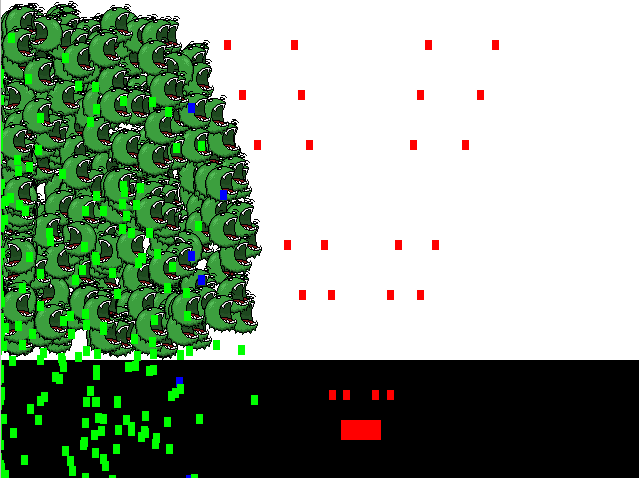
\includegraphics[width=\textwidth]{games/spacemunch/screenshot.png}
\end{figure}


\section{In-Class Examples}
% basic (inheritence?)
% tiefighter
% app framework

\section{Homeworks}
% TODO: do this section

% sample homework
% sample TDD


\section{Tools}
\lstinputlisting[language=bash,%
                 label=lst:turnin,%
                 caption={[turnin.sh] Turnin.sh: A utility script for students to push their homework to github}]
                 {course/turnin.sh}


\section{Advanced Section}
% TODO: description of advanced section

\lstinputlisting[language=Python,%
                 label=lst:pyfactory,%
                 firstline=2,
                 lastline=18,
                 caption={[Enemy Factory] Enemy Factory: A simple example of class/factory methods}]
                 {course/classcode/adv_section/enemy_with_factory.py}

\lstinputlisting[language=Python,%
                 label=lst:pyevtmgr,%
                caption={[Event Manager] Event Manager: An example of using the observer/listener patterns}]
                 {course/classcode/adv_section/event_manager.py}

% TODO: lookup pubsup spelling
\lstinputlisting[language=Python,%
                 label=lst:pysignals,%
                 caption={[Signals] Signals: An example of using pub-sub and the louie API}]
                 {course/samplecode/signals/signals.py}


\section{Final Project Sample Code}

% TODO explain example code
% TODO: link to coinget

% tiles

% text blocks

%\begin{listing}[H]
%  \label{lst:pyg-app}
%  \caption{Application Framework with base State class}
%  \inputminted[linenos]{python}{works/pygame/Super-Coin-Get/coinget/core/app.py}
%\end{listing}
%
%\begin{listing}[H]
%  \label{lst:pyg-collision}
%  \caption{Custom Sprite Collision}
%  \inputminted[firstline=188,lastline=189,linenos]{python}{works/pygame/CS112-Spring2012/samplecode/tiefighter_example/main.py}
%  \inputminted[firstline=60,lastline=61,linenos]{python}{works/pygame/CS112-Spring2012/samplecode/tiefighter_example/main.py}
%  \inputminted[firstline=16,lastline=33,linenos]{python}{works/pygame/CS112-Spring2012/samplecode/tiefighter_example/utils.py}
%\end{listing}

